\chapter{Questsystem}
Eine Quest ist eine Aufgabe, die dem Benutzer gestellt wird. Diese kann in der Quest-Auswahl gewählt werden. Quests sind in so genannten Packages gegliedert. 

Mithilfe des Quest System soll die Motivation und der Lernerfolg der Nutzer gesteigert werden. Durch bewältigte Programmieraufgaben können Schüler hierbei Auszeichnungen bekommen. Weiters wird auch der Lernfortschritt visuell dargestellt.


\section{Unterschiede zur Herkömmlichen Aufgabenverteilung}
Der frühere Unterricht wurde so gestaltet, dass der Lehrer vor der Stunde an die Schüler die Aufgaben austeilte. Diese konnten nun vom Schüler ausgearbeitet werden. Die Aufgaben mussten von der Lehrperson auf Richtigkeit und Vollständigkeit überprüft werden, wodurch auch das selbstständige Lernen erschwert wurde.

Bei diesem System, kann der Schüler direkt aus einem Themenblock auswählen und der Fortschritt wird im Profil vermerkt. Dies hat vor allem dann Sinn, wenn Lehrpersonen überprüfen wollen, ob die Aufgaben erledigt wurden. Wenn der Schüler mit die Aufgabe abgeschlossen hat, kann er sogleich mit der nächsten Quest beginnen. Somit wird der Schüler auch beim selbstständigen Lernen unterstützt.

\section{Dateien in einer Quest}
\begin{figure}[h] 
  \centering
     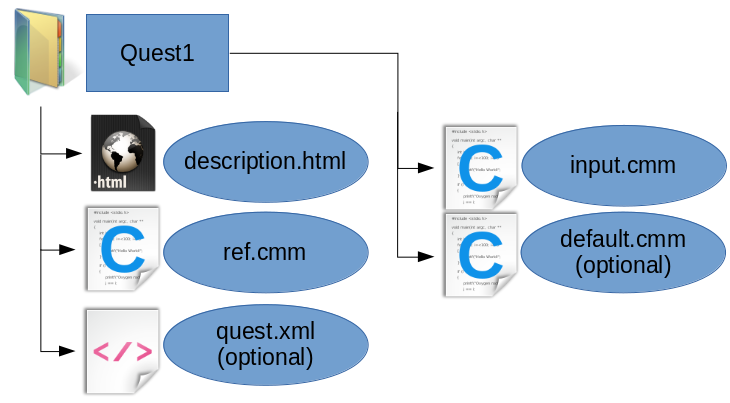
\includegraphics[width=0.8\textwidth]{./media/images/quest/quest_ordnerstruktur}
  \caption{Struktur einer Quest}
  \label{fig:struct_quest}
\end{figure}

Damit eine Quest vom Programm als so welche erkannt wird, müssen mehrere Dateien vorhanden sein. Einige davon werden von der Überprüfungsroutine benötigt. Andere dienen wiederum zur Beschreibung der Quest.

\begin{itemize}
\item description.html\\
Diese Datei beinhaltet die Beschreibung der Quest. Diese muss im .html Format geschrieben werden. Hier kann die Aufgabe ausführlich erklärt werden. Informationen über Tokens müssen manuell in die Beschreibung hinzugefügt werden.

\item ref.cmm\\
In der ref.cmm befindet sich das Referenzprogramm. Dieses wird von C-Compact beim Überprüfen der Quest ausgeführt. Wenn die Ausgaben des Programms des Benutzers, den Ausgaben des Referenzfiles gleichen, wird die Aufgabe als Richtig gewertet.

\item default.cmm\\
In der default.cmm befindet sich eine Quelltext Vorgabe, welche beim erstmaligen öffnen einer Quests angezeigt beziehungsweise zur weiteren Verarbeitung zur Verfügung gestellt wird.

\item input.cmm\\
Dieses File kann zum Erstellen für Eingabedaten der ref.cmm verwendet.
\end{itemize}

Optional können noch weitere Dateien hinzugefügt werden. Wenn diese unvollständig oder kaputt sind, so wird eine dieser Dateien einfach nicht verwendet.

\begin{itemize}
\item quest.xml\\
In diesem File kann man einige Parameter der Quest definieren, diese werden im Quest- Auswahlfenster genutzt.

\begin{lstlisting}[language=XML]
<quest>
    <title>Example-Quest-Name</title>
    <attribute>Übung</attribute>
    <token>example.xml</token>
    <previousFolder>andereQuest</previousFolder>
    <state>locked</state>
</quest>
\end{lstlisting}
Wie aus der Datei bereits ersichtlich sein sollte, kann man einen Titel, ein Attribut, die dazugehörige Auszeichnung und einen Status bestimmen. 
\begin{itemize}
	\item Falls kein Titel gewählt wird, wird automatisch der Ordnername als Titel gewählt. 
\item Sollte kein Attribut gewählt werden, bleibt dieses Feld in der Questauswahl leer.
\item PreviousFolder, dient zum Einstellen einer Quest welche bereits vor dem diese Quest begonnen werden kann, erledigt sein muss.
\item Bei token, kann man eine zugehörige Auszeichnung wählen. Diese muss im zugehörigen Package im tokens Ordner definiert sein. Wenn dieses nicht vorhanden oder Fehlerhaft ist, wird bei Abschluss der Quest, kein Token hinzugefügt.
\end{itemize}
Alle diese hier erwähnten Optionen können optional hinzugefügt werden.
\item style.css\\
Kann als Stylesheet für die dazugehörige description.html verwendet werden. Diese Datei ersetzt das vordefinierte Stylesheet.

\end{itemize}

\section{Variablen in der quest.java}
\begin{lstlisting}[language=JAVA]
//Kann von der quest.xml definiert werden
	private String title;			//Titel der Quest		
	private Token token;			//Referenz zum Token
	private String matcher;			//Reguläre expression, für Auswertung benötigt
	private String state;			//locked, selectable, finished,..
	private String attribute;		//Attribut bei der Questauswahl
	private String previousFolder;	//Muss vorher eine Quest erledigt werden

//Wird durch andere Faktoren bestimmt
	private boolean description;	//Beschreibung
	private boolean style;			//extra Stylesheet
	private boolean ref;			//ref.cmm vorhanden?
	private boolean input;			//input.cmm vorhanden?	
	private boolean defaultCmm;		//default.cmm vorhanden?
	private String cmmFilePath;		//Pfad zum dazugehörigen File	
	private Date date;				//Datum der letzten Bearbeitung
	private String initPath;		//auch "packages"
	private String packagePath;		//Pfad des Packetes
	private String questPath;		//Questordner vom Packet aus

\end{lstlisting}
Alle hier erwähnten Variablen sind durch Getter und Setter erreichbar.


\section{Questzustände}
\begin{itemize}
\item locked:\\ Diese Quest kann nicht bearbeitet werden. Quest wird automatisch auf diesen Zustand gesetzt, falls in der \textit{quest.xml} für \textit{\textbf{previousFolder}} ein Wert gesetzt wurde, und dieser Wert im Profil noch nicht als fertiggestellt markiert wurde.
\item selectable:\\ Der Benutzer kann diese Quest auswählen. Dies hier ist der Standartzustand.
\item inprogress:\\ Der Benutzer hat diese Quest bereits begonnen, jedoch noch nicht abgeschlossen.
\item open:\\ Diese Quest wird gerade vom Benutzer bearbeitet.
\item finished:\\ Die Quest wurde bereits abgeschlossen.
\end{itemize}

\section{Linearer Quest Weg}
In so gut wie allen Spielen, von denen sich unser Quest-System ableitet gibt es einen Quest Tree.
Das bedeutet, dass bestimmte Quests erst sichtbar werden, wenn man die Vorgängerquests
abgeschlossen hat. Auf diese Weise kann der Spieler eine Entwicklung erleben und wird unbemerkt
durch die Hintergrundgeschichte des Spieles geführt. In unserem Fall wäre ein Quest tree für den
Lernfortschritt sehr förderlich, da der Benutzer Schritt für Schritt immer komplexere und
anspruchsvollere Aufgaben meistern muss.

Ein Linearer Weg wie man die Quests abarbeiten kann ist bereits vorgesehen: Der Ersteller kann selbst entscheiden, ob man bevor man eine schwierigere Quest starten kann, eine einfachere vorher abschließen muss. In unserem Fall ist der lineare Quest Weg sehr förderlich, da der Benutzer Schritt für Schritt immer komplexere und anspruchsvollere Aufgaben meistern muss.